\documentclass{subfiles}[../main.tex]

\begin{document}

\section{Résultats}
    Afin d'évaluer l'efficacité des états d'essai à trouver l'énergie minimale,
    on peut les comparer à des états d'essai généraux déjà implémentés dans
    Qiskit. À titre de référence, l'énergie minimale calculé par diagonalisation
    exacte était de $-21t$. Pour commencer, on peut comparer le premier état
    d'essai aux états fournis par Qiskit, soit

\begin{figure}[H]
    \begin{center}
        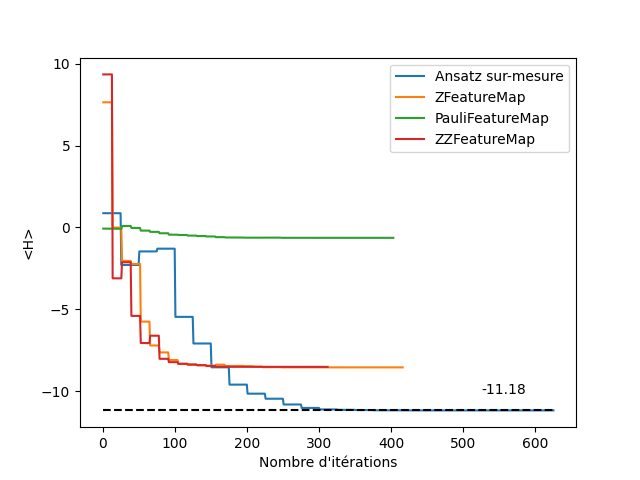
\includegraphics[width=0.95\textwidth]{../figs/convergence.png}
    \end{center}
    \caption{Comparaison de la convergence des états d'essai sur la valeur
    minimale de l'énergie. La valeur minimale obtenue en utilisant le premier
    état d'essai bâti est de $-11.2t$.}
    \label{fig:}
\end{figure}
    Tel qu'attendu, l'état d'essai basé sur la physique du problème converge
    à une énergie plus basse que les autres. Ceci peut être du au fait que
    l'état d'essai utilisé est exprimé en fonction de $2$ fois plus de
    paramètres que ceux de Qiskit. On pourrait augmenter le nombre de paramètres
    des états d'essai fournis par Qiskit en simplement répétant plusieurs fois
    le circuit en introduisant des paramètres supplémentaires. Cependant, ceci
    augmente la profondeur du circuit de manière considérable, tandis que les
    portes quantiques utilisé dans le premier état d'essai développé sont toutes
    implémentable par un ou quelques pulses sur un véritable ordinateur quantique. Comme
    la profondeur du circuit joue un rôle important dans la qualité de l'état
    préparé, il s'agit de balancer le nombre de paramètres et la profondeur
    du circuit pour assurer le meilleur rendement.\\
    Maintenant que l'énergie du fondamental calculé en utilisant l'état d'essai bâti
    précédemment donne une énergie plus basse que ceux fournis par Qiskit, il est
    intéressant de le comparer au deuxième état d'essai bâti.

\begin{figure}[H]
    \begin{center}
        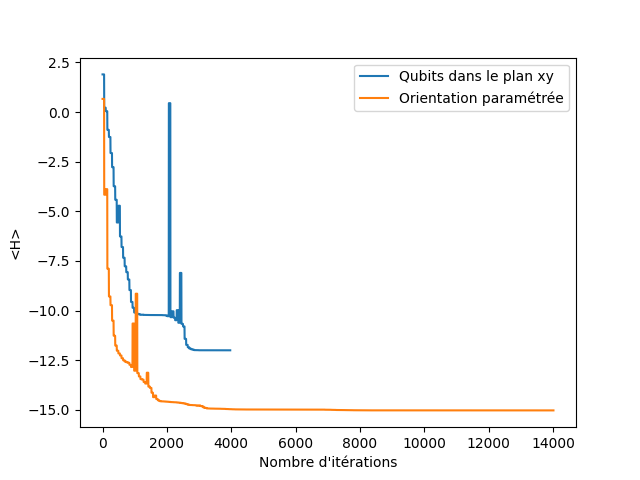
\includegraphics[width=0.95\textwidth]{../figs/convergence_upgrade.png}
    \end{center}
    \caption{Comparaison entre les deux état d'essai "maison". Tel qu'attendu,
    celui avec d'avantage de degrées de liberté permet de trouver une énergie
    minimale plus petite. Le minimum atteint est de $-15t$.}
    \label{fig:}
\end{figure}
    Tel qu'on peut le voir, en ajoutant la liberté aux qubits d'avoir une inclinaison
    par rapport au plan $O_{xy}$ sur la sphère de Bloch, il est possible d'obtenir
    une erreur de $30\%$ sur l'énergie minimale (comparée à la diagonalisation
    exacte.) Cette comparaison montre l'effet qu'a le nombre de degrées de liberté
    accordé à l'état d'essai sur la valeur de l'énergie du fondamental. En
    augmentant le nombre de degrés de libertés indépendants à l'état, il est
    certain que le minimium absolu de la valeur moyenne de l'hamiltonien diminue
    ou reste constant. Le problème est alors dans l'algorithme classique d'optimisation.
    Avec $2$ fois plus de paramètres, le second état d'essai mène à une énergie
    en fonction de $48$ paramètres. Il serait intéressant d'explorer les
    algorithmes classique d'optimisation afin de définir une limite idéale au
    nombre de paramètres à considérer.\\
    Naturellement, on pourrait penser qu'en ajoutant autant de paramètres que l'on
    souhaite on arrive à une énergie de plus en plus près de l'énergie exacte.
    Or, plusieurs autres états d'essai ont été essayés avant et après avoir bâti
    ceux présenté qui n'admettait pas une énergie plus basse que ceux-ci. Ceci
    est du au manque d'exploration du domaine en partie, mais probablement plus
    au fait que les paramètres ajoutés était soit redondant ou des paramètres qui
    n'influence pas l'énergie. Étant donné la haute dégénérescence d'un liquide
    de spin, il est fort probable qu'il s'agit de la seconde option, car le
    nombre de dégénérescence est égale au nombre de degrés de liberté qui
    n'influence pas la valeur de l'énergie du fondamental.

\end{document}
